% Document Class is specified here. We're using the Homework Template
\documentclass[12pt, a4paper]{article}

\usepackage{graphicx}
\usepackage{float}
\usepackage{geometry}
\usepackage{verbatim}

\geometry{a4paper, margin=1in}

\title{Week 2 CS-312 Homework}
\author{
	Cory Ness
	\and
	Jack Engledow
	\and
	James Sgrazzutti
}

\begin{document}

\maketitle

\section{Problem 1.11}
\subsection{Question}
Construct an FA that accepts all binary strings with precisely three 1's.
\subsection{Answer}
\begin{center}
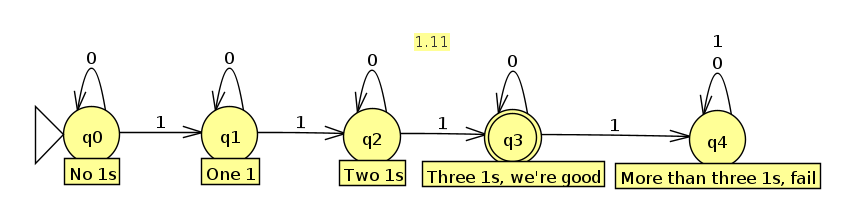
\includegraphics[scale=0.3]{1.11}
\end{center}

\section{Problem 1.13}
\subsection{Question}
Give an FA for the language of all binary strings that have at least three symbols and whose first and last symbols are different.
\subsection{Answer}
\begin{center}
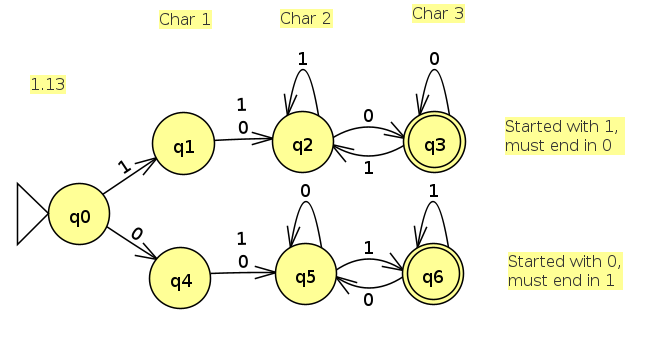
\includegraphics[scale=0.3]{1.13}
\end{center}

\section{Problem 1.15}
\subsection{Question}
Construct an FA that accepts all strings of $\{a, b\}$ that contain either $ab$ or $bba$ (or both) as substrings.
\subsection{Answer}
\begin{center}
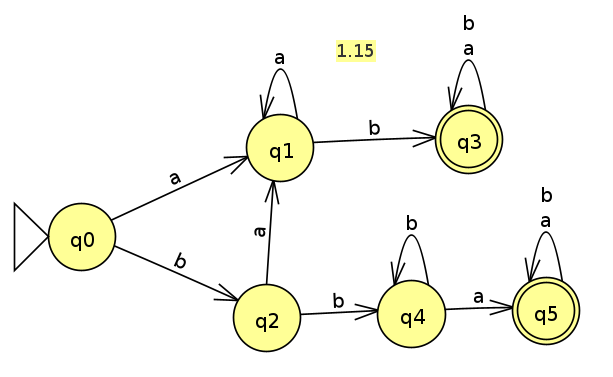
\includegraphics[scale=0.3]{1.15}
\end{center}

\section{Problem 1.17}
\subsection{Question}
Construct an FA that accepts all binary strings with an even number of $0$'s and the number of $1$'s is a multiple of 3.
\subsection{Answer}
\begin{center}
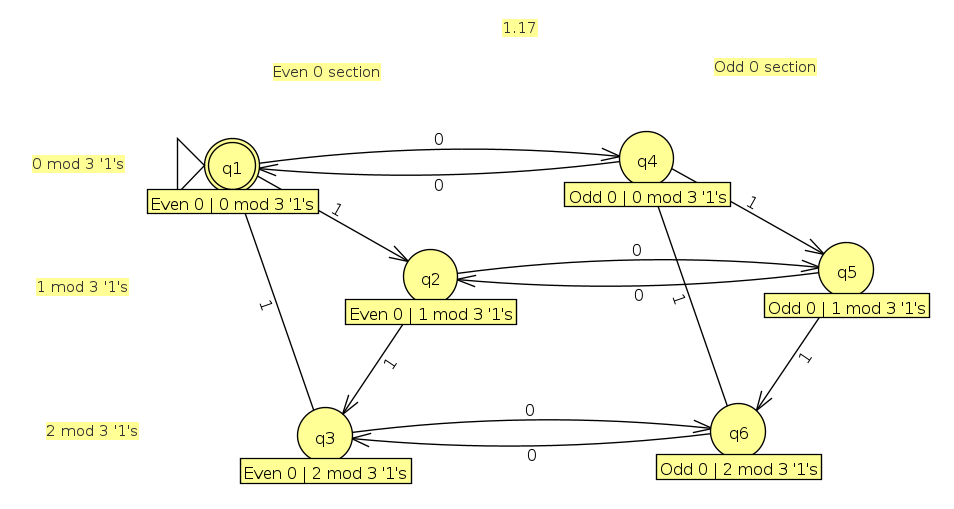
\includegraphics[scale=0.3]{1.17}
\end{center}

\section{Problem 1.19}
\subsection{Question}
Explain in English what the following FA accepts:
\begin{center}
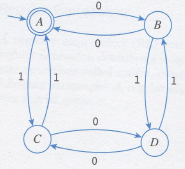
\includegraphics[scale=1]{1.19-problem}
\end{center}
\subsection{Answer}
The FA accepts any binary string with an even number of $0$'s and an even number of $1$'s.

\section{Problem 2.3}
Give RE's for:
\subsection{All binary strings with exactly two R$1$'s}
\begin{center}
\verb@0*10*10*@
\end{center}
\subsection{All binary strings with a double symbol (contains $00$ or $11$) somewhere}
\begin{center}
\verb@(0+1)*(00+11)(0+1)*@
\end{center}
\subsection{All binary strings that contain both $00$ and $11$ as substrings}
\begin{center}
\verb@(0+1)*((00(0+1)*11)+(11(0+1)*00))(0+1)*@
\end{center}
\subsection{All binary strings without a double symbol anywhere}
\begin{center}
\verb@((01)*(!+0))+((10)*(!+1))+0+1+!@
\end{center}

\section{Problem 2.7}
\subsection{Question}
Give an RE for the language of Exercise 1.12
\subsection{Answer}
\begin{center}
\verb@((b+c)*+((b+c)*a(b+c)*a(b+c)*)*)a(b+c)*@
\end{center}

\section{Problem 2.10}
\subsection{Question}
Give an RE for the language of Exercise 1.15
\subsection{Answer}
\begin{center}
\verb@(a+b)*((ab)+(bba))(a+b)*@
\end{center} 	

\section{Problem 2.15}
\subsection{Question}
Show that the language of RE\verb@(0*1*)*@ is all binary strings.
\subsection{Answer}
We can trivially prove that the Regular Expression accepts all binary strings if we were to look at the Discrete Finite Automata equivalent. In order to get there, we first perform a Nondiscrete Finite Automata  conversion, creating the graph shown below.
\begin{center}
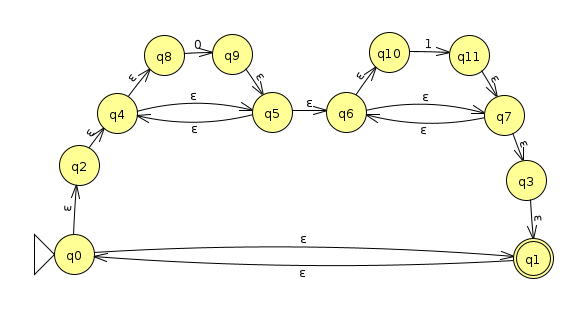
\includegraphics[scale=0.5]{2.15NFA}
\end{center}
From here, we can convert it into a Discrete Finite Automata, seen below.
\begin{center}
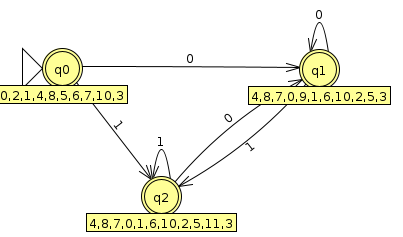
\includegraphics[scale=0.5]{2.15DFA}
\end{center}
And from here we can trivially see the DFA accepts any binary string, including the empty string. This is because it initializes to a final state, and transitions to a final state on 0 or 1, regardless of the previous state, hence any binary string is accepted by this DFA.

\end{document}